\section{Methods}
\begin{frame}{The Stiffness Problem}
    \begin{columns}
        \begin{column}{0.4\textwidth}
        \Large
            $^1$H Fusion \textcolor{blue}{$\lambda$}: \\ 7.90 $\times$ 10$^{-20} \frac{\mathrm{cm}^3}{\text{mol s}}$\\ \vspace{20pt}
            $^2$H Fusion \textcolor{blue}{$\lambda$}: \\ 1.01 $\times$ 10$^{-1} \frac{\mathrm{cm}^3}{\text{mol s}}$
        \end{column}
        \begin{column}{0.6\textwidth}
            \begin{figure}
                \centering
                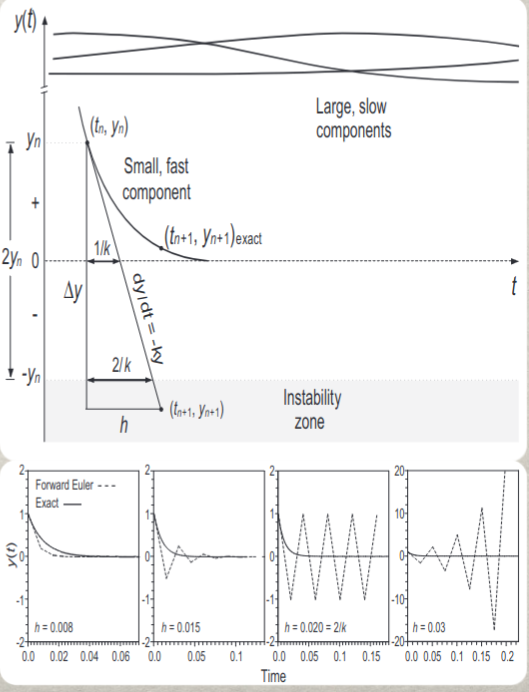
\includegraphics[width = 0.75\textwidth]{figs/hix.png}
                \caption{ Explicit methods destroy solutions for stiff equactions \\Source: W.R. Hix}
                \label{fig:enter-label}
            \end{figure}
        \end{column}
    \end{columns}
\end{frame}
\begin{frame}{Implicit Euler \& Newton-Raphson}
    \begin{gather*}
        \only<1-4>{
            \frac{Y_{n+1}- Y_n}{\Delta t} = \dot{Y}_{n+1} \\
        }
        \only<2-4>{
        \frac{Y_{n+1} - Y_n}{\Delta t} - \dot{Y}_{n+1} = 0 \\
        }
        \only<3-4>{
        F(Y_{n+1}) = 0 \rightarrow \text{Solve!}
        }
    \end{gather*}
    \only<4>{
    Through Newton-Raphson!
        \begin{gather*}
            Y_{n+1} = Y_n - \left[ J_F(Y_n) \right]^{-1}  F(Y_n), \hspace{10pt} (J_F)_{ij} = \frac{\partial \dot{Y}_i}{\partial Y_j} - \frac{\delta_{ij}}{\Delta t} 
        \end{gather*}
    }
    \only<5>{
        \begin{figure}
            \centering
            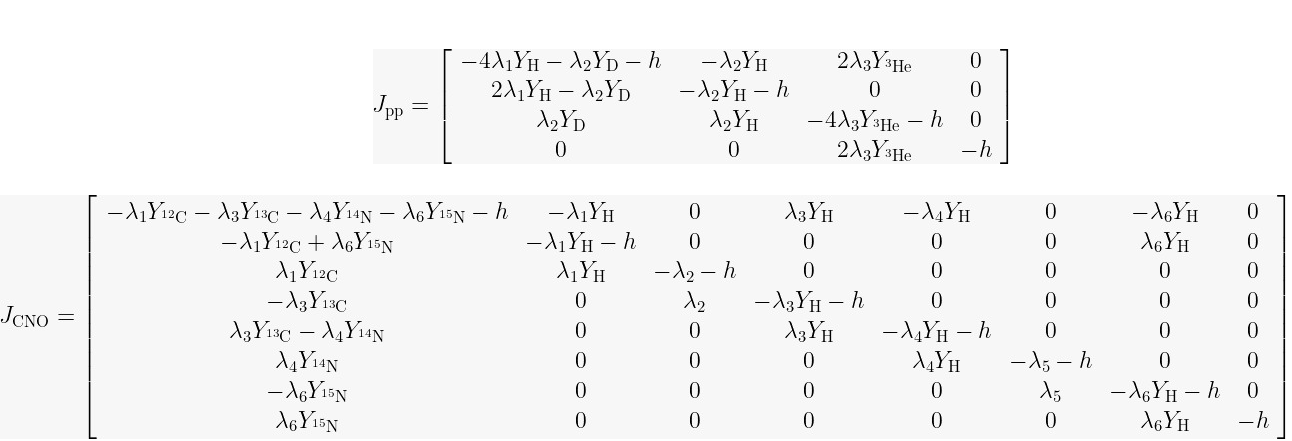
\includegraphics[width = \textwidth]{figs/unhinged_jacobian.png}
            \caption{Jacobians, by hand. Yeah...}
            \label{fig:enter-label}
        \end{figure}
    }
\end{frame}
\begin{frame}{Flow chart}
\begin{figure}
    \centering
    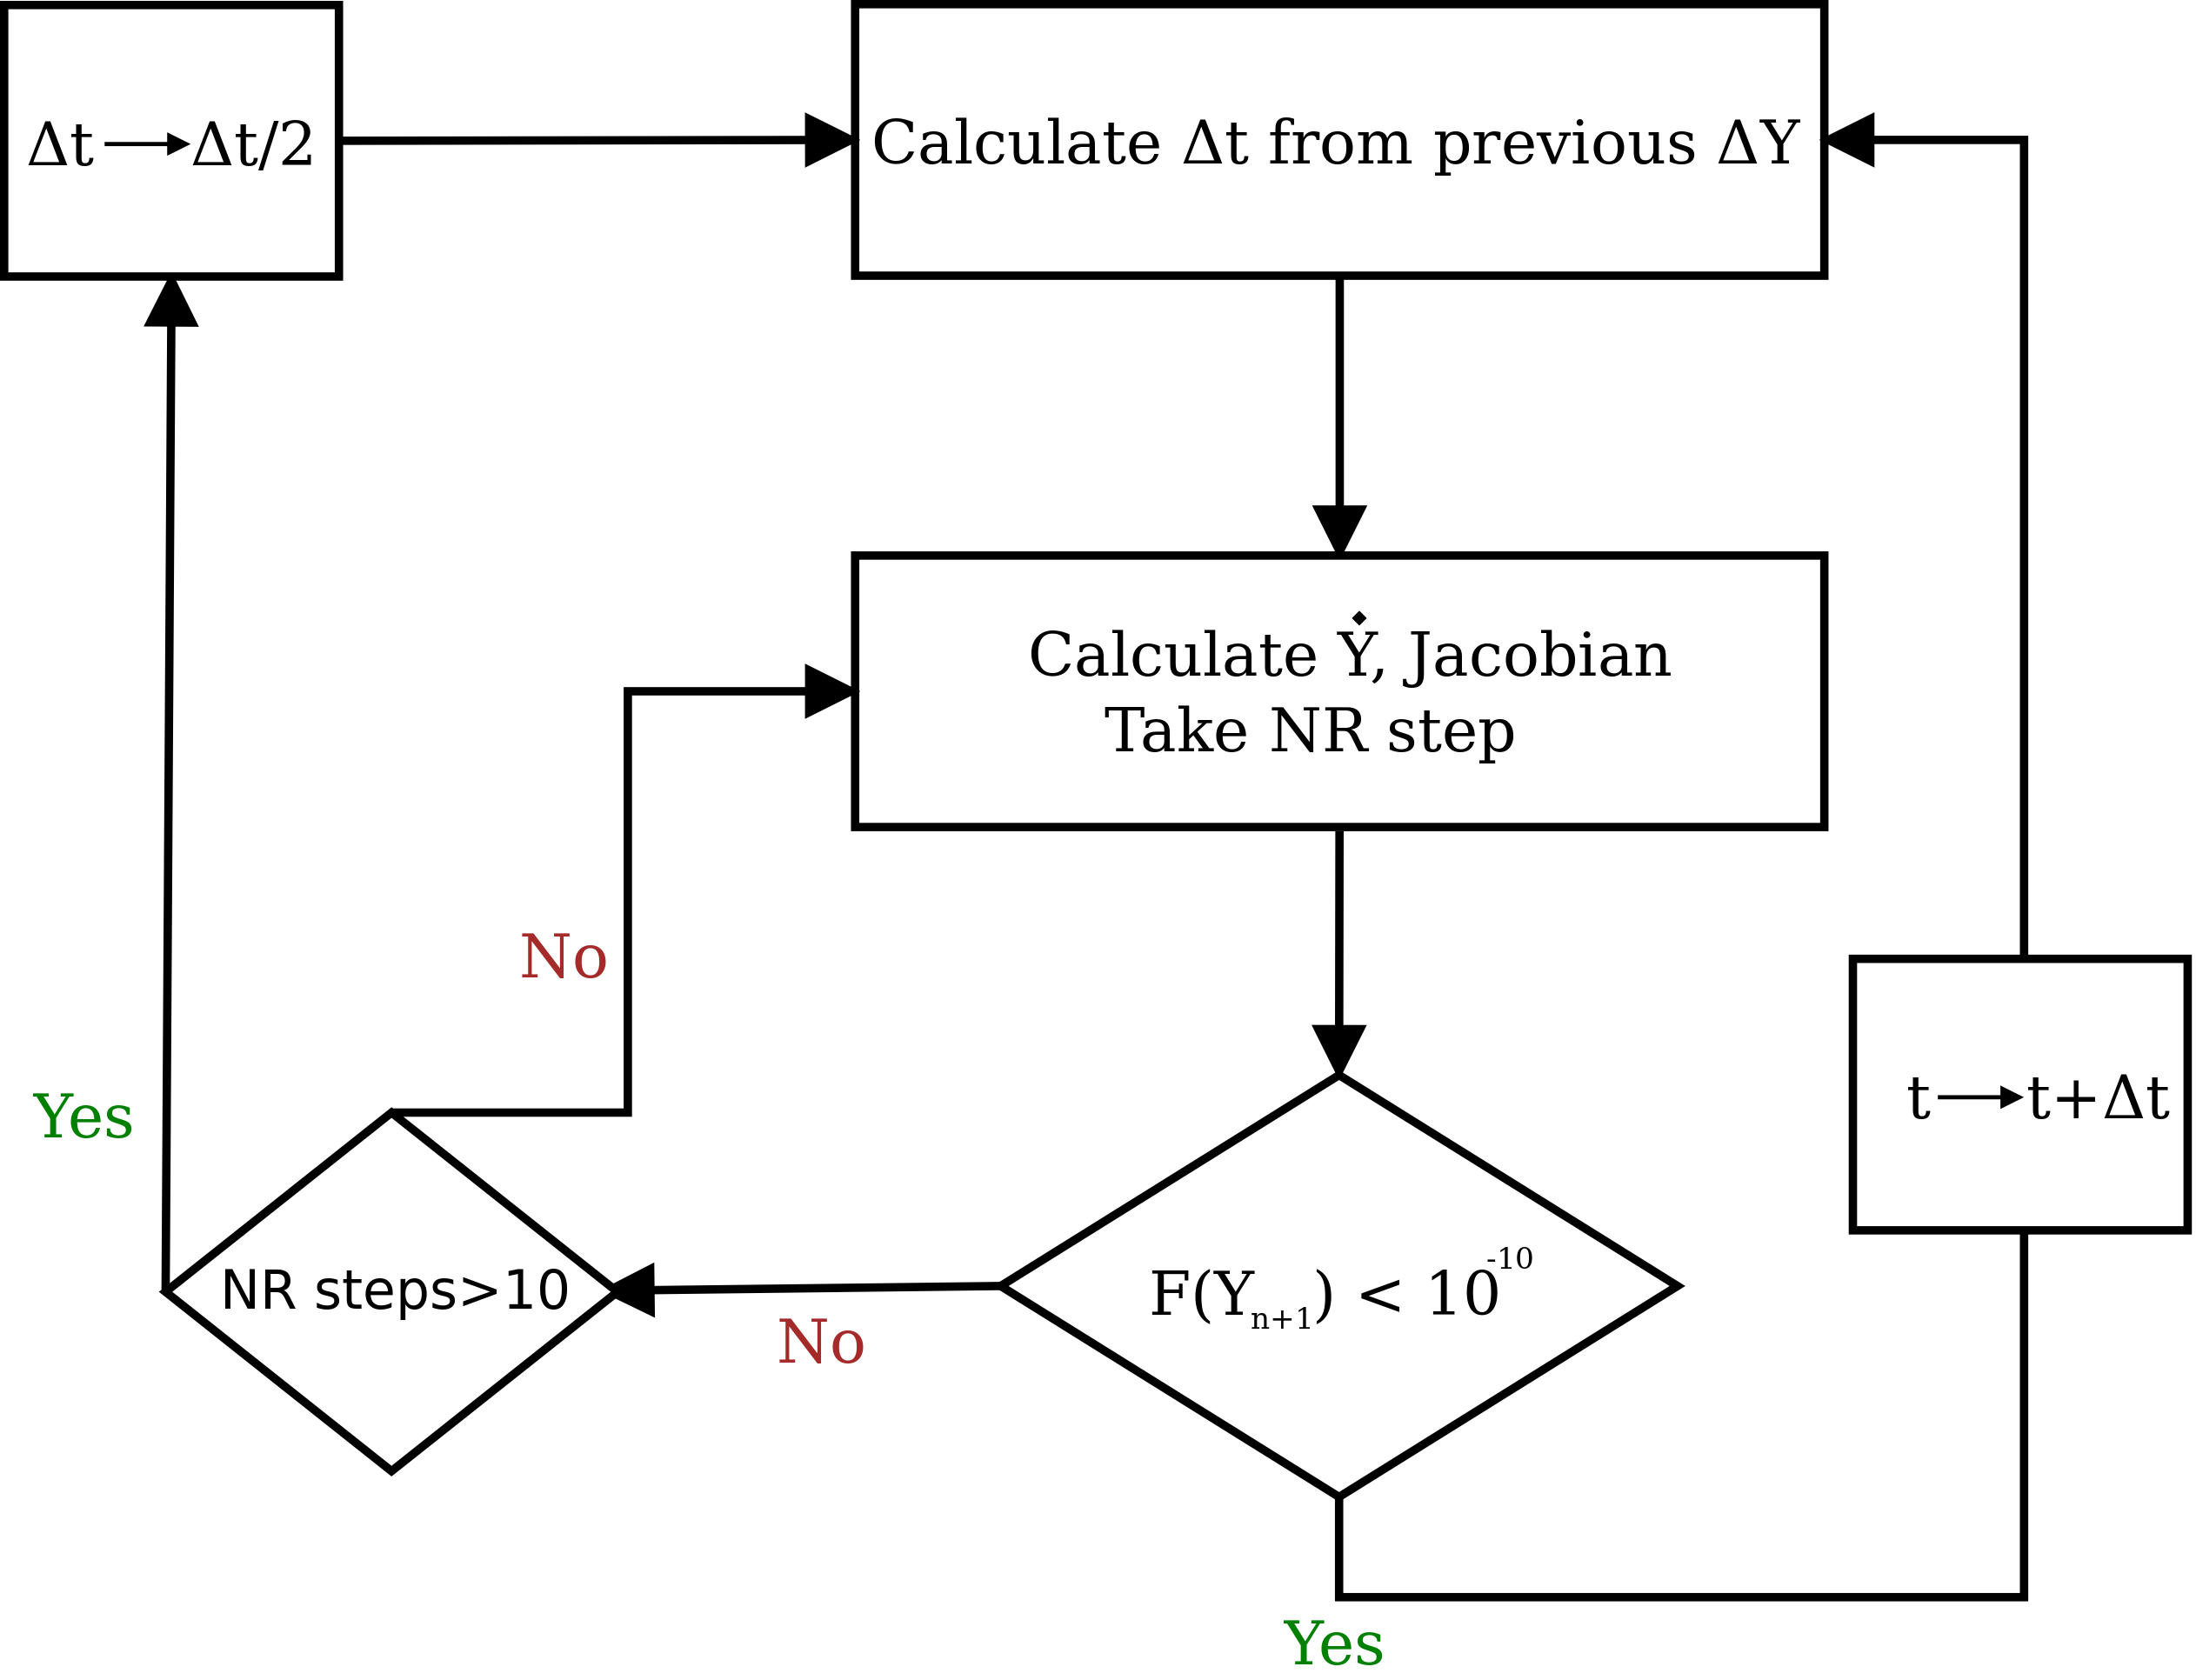
\includegraphics[scale = 0.3]{figs/nrn.png}
    \caption{Flow chart of our NRN. Based on \texttt{SkyNet} Lippuner \& Roberts '18}
    \label{fig:enter-label}
\end{figure}
\end{frame}
\begin{frame}{Initial Conditions \& Assumptions}
\Large
    \begin{itemize}
        \item<1-> $T_\mathrm{core}$, \textcolor{orange}{$\rho$} are constant. No mixing. \\
        \texttt{MESA} simulations to get typical values. 
        \item<2-> $\rho = f(T_\mathrm{core})$
        \item<3-> Constant \textcolor{blue}{$\lambda$}.\\ Thermonuclear from Angulo+'99, Beta decays Kondev+'21
        \item<4-> Initial \textcolor{red}{$Y$} from ISM, unless provided explicitly. Full citations in the \texttt{README}.
    \end{itemize}
\end{frame}